\section{Appendix}

\subsection{Angular correction}

  Because our straws don't in fact measure U and V coordinates directly, but instead distance of closest approach radii deriving from measured hit times, in order to utilize the minimization procedure on measured track parameters these radii must first be converted to U and V parameters. (And similarly for the U and V errors.) (Note that the future Kalman filter will not be subject to this disadvantage.) This is done in the calcMeasuredParams method at the bottom of the GeaneReco module. The wires that are hit as well as the initial raw measured errors are stored indefinitely, and it is upon these objects that corrections are made. These corrections will be dependent on the angle of the track, so it's imporant to note that during each successive iteration, the ``measured'' parameters are adjusted by the latest ``predicted'' momenta. It was found that for the error correction, a simple straight line correction was sufficient for ideal results. For the position correction, it was found that a constant field correction for curved tracks was sufficient.

  To calculate these corrections, first the momentum perpendicular to the straw measurement axis can be ignored. Because the positron tracks curve in only one direction through the tracker, one needs to calculate the correction depending on whether the track went to the left or right side of the wire. See Figure \ref{fig:angularCorrection} for a pictorial representation of the problem. The calculation of the right side correction follows, with the left side correction being calculated in a similar manner.

\begin{figure}[]
\caption{Shown here is a positron passing through a straw. The desire is to convert the measured parameter d into a U or V position, which can be done by approximating the particle trajectory as a circle in a constant magnetic field over the course of the straw and using trigonometry. Sizes and angles are exaggerated.}
\centering
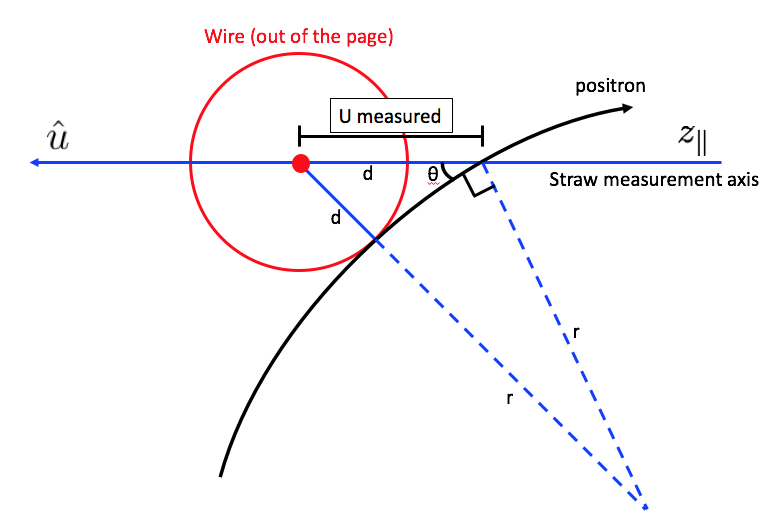
\includegraphics[width=1.0\textwidth]{angularCorrection}
\label{fig:angularCorrection}
\end{figure}

An equation with the single unknown parameter being of interest can by approximated by
$$(r+d)^{2} = r^{2}+u^{2}-2ru\cos(90+\theta),$$ where the 90 degrees is approximate for large curvature of tracks , and we want to solve for u. The angle $\theta$ can be determined from 
$$\hat{z_{\parallel}} \cdot \hat{p_{\parallel}} = \cos{\theta}, \theta = \cos^{-1}{\frac{p_{\parallel}}{p}},$$ where p parallel is the momentum parallel to the z parallel axis at the wire plane and can be determined within the code. Using a trig identity and solving for u gives
$$u = -r\sqrt{1-(\frac{p_{\parallel}}{p})^{2}} + \sqrt{d^{2} + 2dr + r^{2}(1-(\frac{p_{\parallel}}{p})^{2})},$$ for the right side correction, and 
$$u = +r\sqrt{1-(\frac{p_{\parallel}}{p})^{2}} - \sqrt{d^{2} + 2dr + r^{2}(1-(\frac{p_{\parallel}}{p})^{2})},$$ for the left side correction. (Corrections to v are identical.) The radius of the particle circle can be calculated from the circular momentum and magnetic field at the predicted hit position. The straightline correction is done simply using the Pythagorean theorem in a simpler manner, with the correction to the errors then being
$$\sigma_{uv}' = \frac{\sigma_{uv}}{\sqrt{1-(\frac{p_{\parallel}}{p})^{2}}}$$.

